% arara: setup
% arara: lualatex: {options: ["--output-directory=build"]}
% arara: lualatex: {options: ["--output-directory=build"]}
% arara: lualatex: {options: ["--output-directory=build"]}
% arara: move: {files: ["build/cover.pdf"], target: "cover.pdf"}
\documentclass{article}

\RequirePackage{pdfmanagement}\SetKeys[document/metadata]{pdfversion=1.7,pdfstandard=a-3b}

\usepackage{fontspec}
\usepackage{geometry}
\usepackage{graphicx}
\usepackage{lipsum}
\usepackage{enumitem}
\usepackage{microtype}
\usepackage{pdfpages}
\usepackage{tikz}
\usepackage{xcolor}

\usetikzlibrary{calc,fadings}

\setmainfont{Libertinus Serif}
\setsansfont{Libertinus Sans}

\definecolor{coverbg}{HTML}{1A1F2C}
\definecolor{chapgold}{HTML}{D1A86F}

\newlength{\spinewidth}\setlength{\spinewidth}{10mm}

\geometry{paperwidth=\dimexpr 382mm+\spinewidth\relax,paperheight=280mm,margin=0mm}

\def\frontshift{\dimexpr 206mm+\spinewidth\relax}

\begin{document}
\pagecolor{coverbg}
\color{white}
\begin{tikzpicture}[remember picture,overlay]
    \fill[coverbg]
        (current page.north west) rectangle ([yshift=140mm] current page.south east);
    \fill[coverbg,path fading=south]
        ([yshift=140mm] current page.south west) rectangle ([yshift=90mm] current page.south east);
    \shade[left color=coverbg,right color=coverbg!85!black]
        ([xshift=191mm] current page.north west) rectangle ([xshift=\dimexpr 191mm+0.5\spinewidth\relax] current page.south west);
    \shade[left color=coverbg!85!black,right color=coverbg]
        ([xshift=\dimexpr 191mm+0.5\spinewidth\relax] current page.north west) rectangle ([xshift=\dimexpr 191mm+\spinewidth\relax] current page.south west);
    \node[rotate=-90,font=\large\sffamily] at ([yshift=0mm] current page.center) {
        \makebox[195mm]{Prague 2026\hfill\textbf{DISSERTATION}\hfill Ing. Tomáš Jíra}
    };
    \node[inner sep=0pt,anchor=center,yshift=-100mm] (wave) at (current page.center) {
        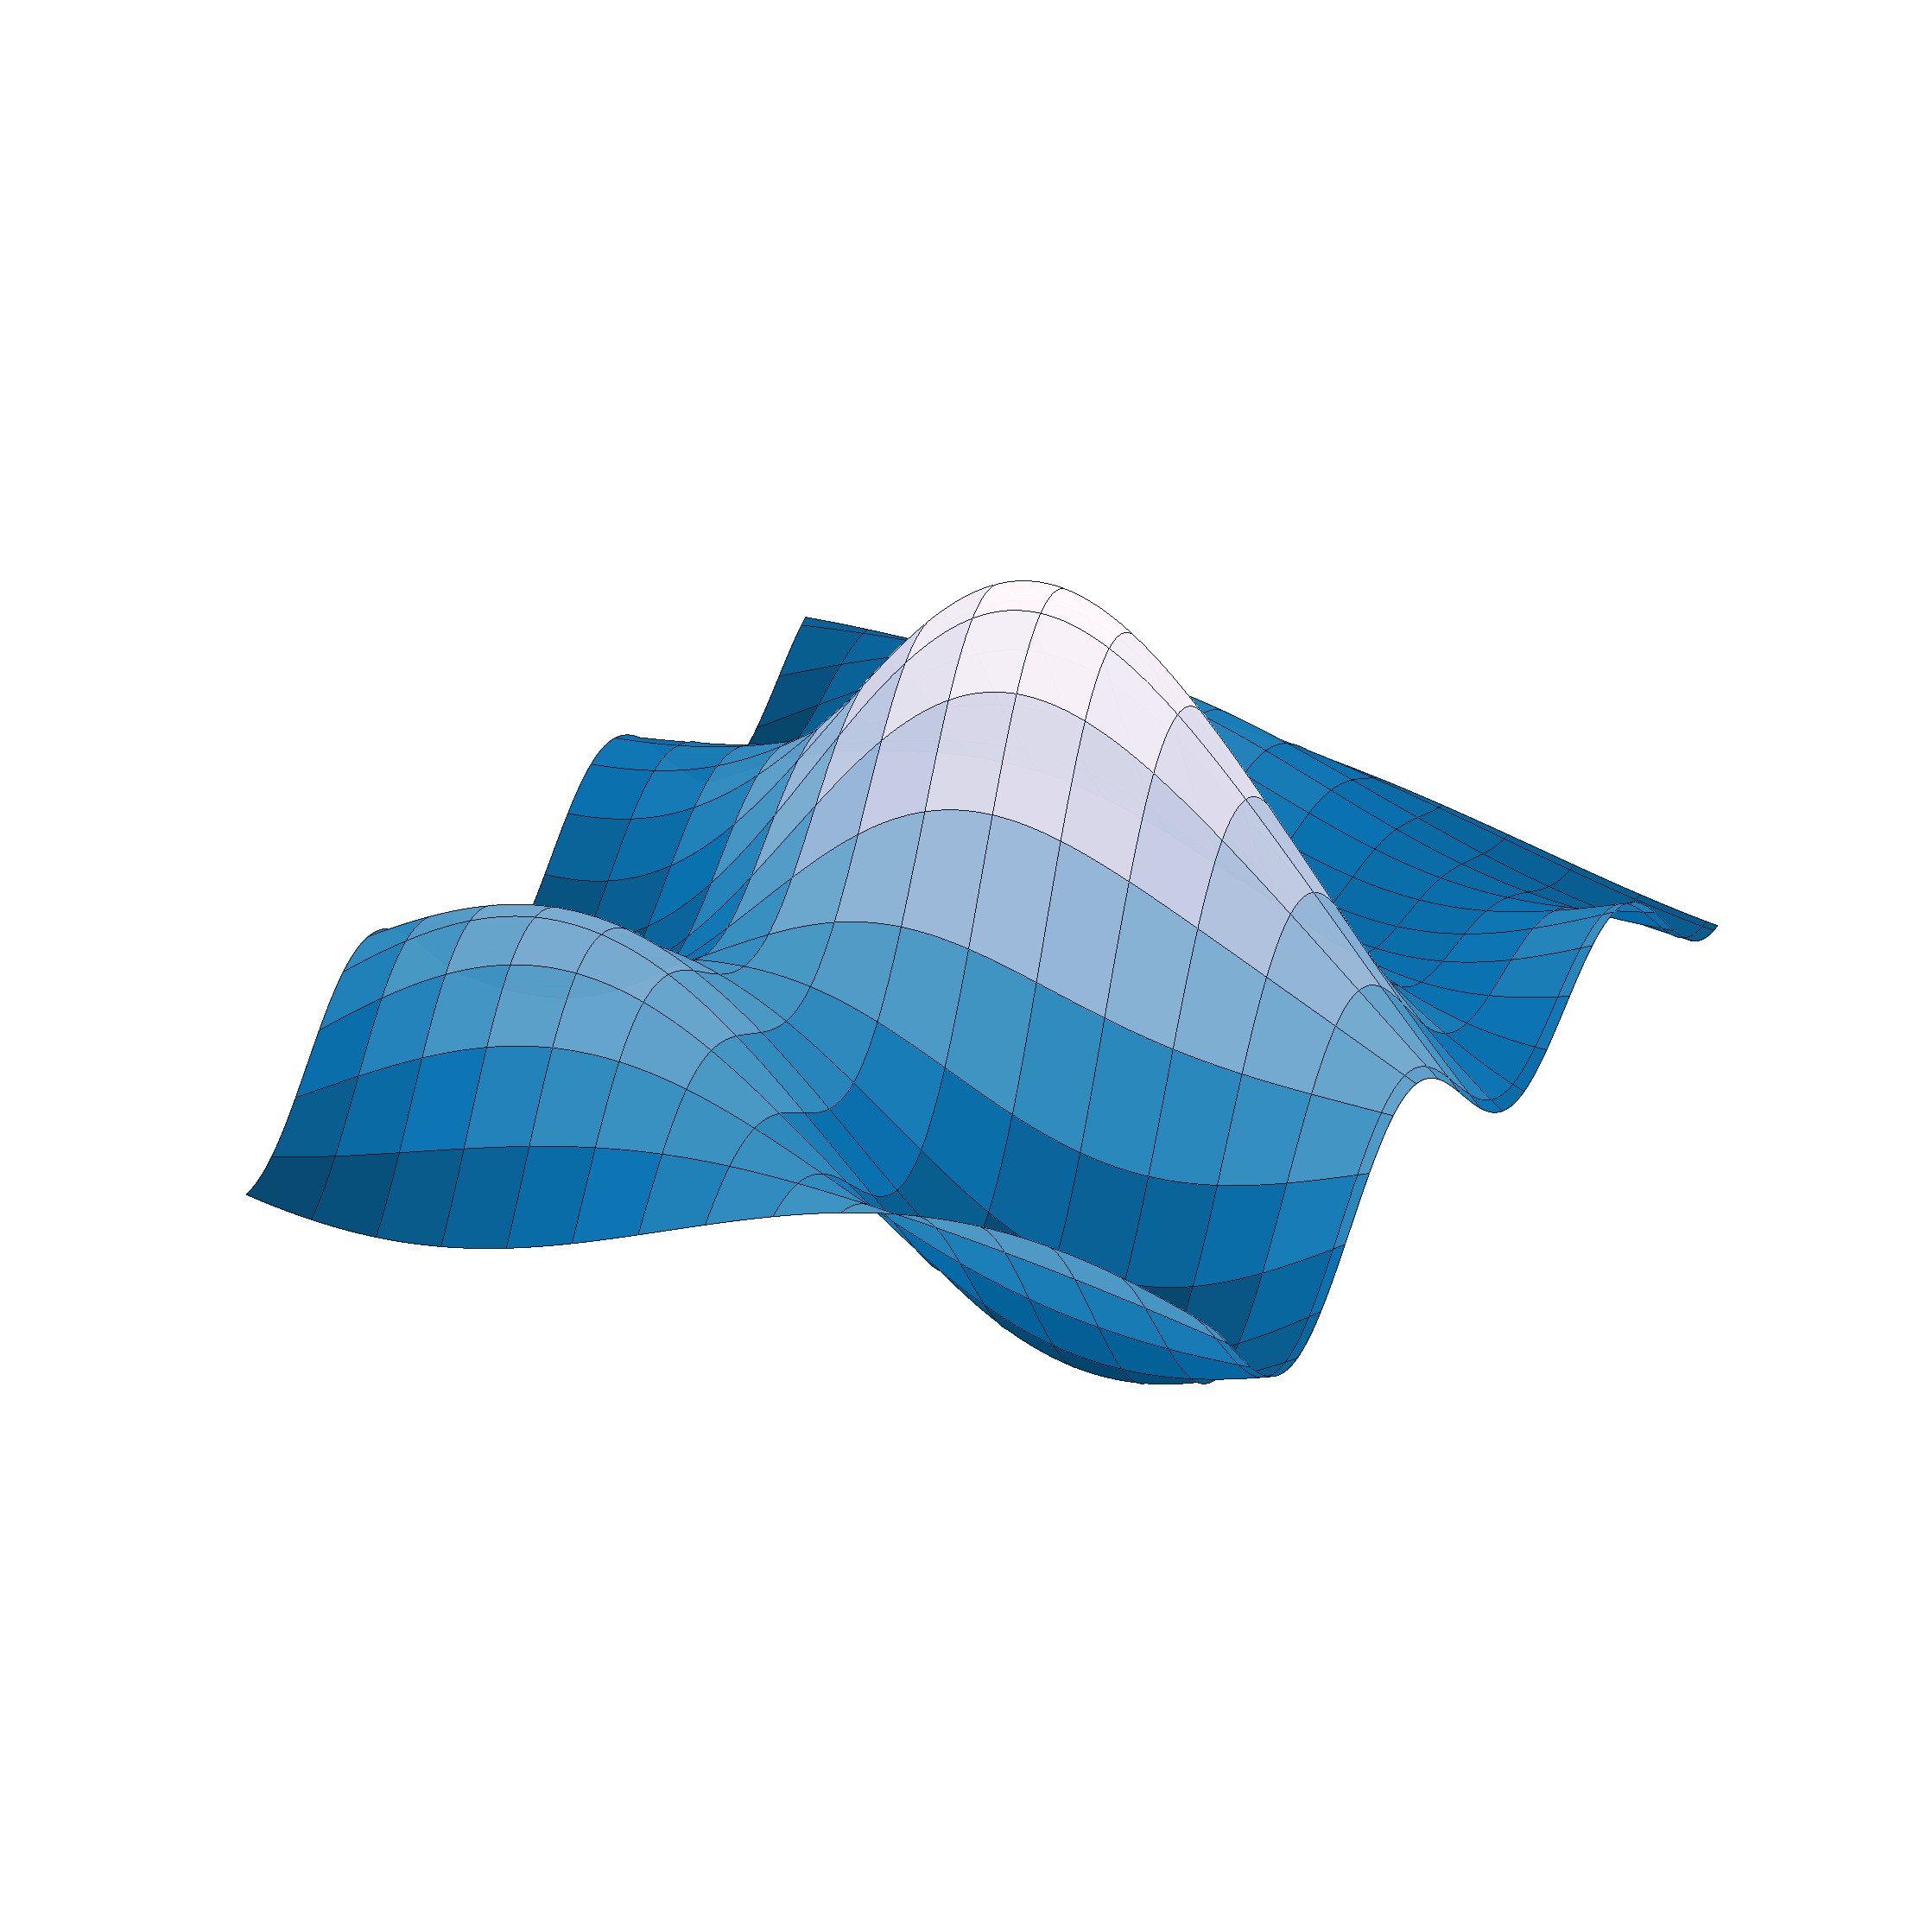
\includegraphics[width=600mm,height=260mm,trim={3.95cm 0 3.05cm 0},clip]{frontmatter/pdf/wave.pdf}
    };
    \node[anchor=north west,inner sep=0pt] at ([xshift=\frontshift,yshift=-50mm] current page.north west) {
        \begin{minipage}[t]{146mm}
            \raggedright
            {\sffamily\normalsize\color{chapgold}\textls[80]{\uppercase{University of Chemistry\\and Technology Prague}}\\[3mm]}
            {\sffamily\normalsize\uppercase{Faculty of Chemical Engineering}\\[25mm]}
            \begin{tikzpicture}
                \shade[left color=chapgold!80!black,right color=chapgold!80!black,middle color=white!80!chapgold] (0,0) rectangle (146mm,7pt);
            \end{tikzpicture}\\[4mm]
            {\fontsize{32pt}{36pt}\selectfont\textbf{Computational Strategies\\[2mm]for Nonadiabatic\\[2mm]Molecular Dynamics}\\[6mm]}
            
\begin{tikzpicture}
                \shade[left color=chapgold!80!black,right color=chapgold!80!black,middle color=white!80!chapgold] (0,0) rectangle (146mm,7pt);
            \end{tikzpicture}\\[20mm]
            {\sffamily\large\color{chapgold}\textls[150]{\uppercase{Dissertation}}\\[5mm]}
            {\fontsize{24pt}{28pt}\selectfont\textbf{Ing. Tomáš Jíra}\\[3mm]\normalsize Prague 2026}
        \end{minipage}
    };
\end{tikzpicture}
\end{document}
